\chapter{Optimizing Object Model and Calls}
\label{chp:ch6-object}

Python is an object oriented programing language.
It is a common practice for programmers to encapsulate state and logic using classes in Python programs.
As an implementation of the Python language, it is essential for us to ensure the performance of object operations and method calls in ZipPy.
In the previous chapters we discussed how we optimize arithmetics (Chapter~\ref{chp:ch4-zippy}) and accelerate iterators (Chapter~\ref{chp:ch5-peeling}).
In this chapter we explain how we implement object operations and calls in ZipPy.

\section{Object Model}
\label{sec:ch5-object-module}

\subsection{Python Object Data Representations}

In Python all data is an object.
CPython, the original implementation of Python, constructs every data type in Python as a heap allocated data structure.
Since it is written in C, CPython implements Python built-in data types using C struct and user defined types using hash maps.
This model results in expensive arithmetic operations due to frequent accesses and allocations of data structures in the heap.
Hash map based object model is also inefficient.
Although the cost of hash map operations is amortized for large data sets, the overhead of retrieving or updating a single map entry is still expensive.
In a hash map based object model, retrieving the value of an object field, or an object attribute in Python, is equivalent to reading the value of a map entry.
This operation involves a hashing calculation and a few steps of memory accesses before reaching the memory address that stores the target value.
On the other hand, in a traditional programming language like Java, an object field access, if optimized, is simply a single memory read.
In summary, object model inefficiency is the main impediment to the performance of popular dynamic languages like Python.

\subsubsection{Jython's Object Model Design}

Existing JVM based Python implementations like Jython, however, replicate the same object model design we saw in CPython.
The main approach they took is porting the existing design from C to Java hoping that the underlying Java compiler will magically optimize it.
This approach failed to realize that, although, the Java JIT compiler is powerful, its strength is in compiling and optimizing programs written in Java,
the first class citizen of the JVM.
Hence, without additional knowledge to the guest language, the Java compiler is unable to address the miss match between the object model of the guest language and Java in an efficient way.
A more efficient solution requires identifying the strengths of the Java compiler and mapping critical components of the guest language onto efficient constructs offered of the JVM.
In the rest of this Section, we describe how we close the gap between the object models of Python and the JVM in ZipPy.

\subsubsection{Multiple Data Representations}

\begin{figure}
\centering
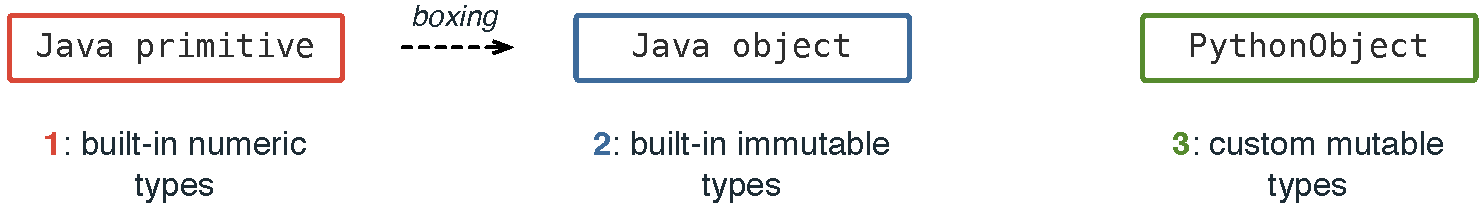
\includegraphics[scale=.6]{figures/ch5-three-data-representations}
\caption{Three data representations for Python objects}
\label{fig:ch5-three-data-representations}
\end{figure}

ZipPy internally uses multiple data representations to model Python objects.
Figure~\ref{fig:ch5-three-data-representations} illustrates this design scheme.
The descriptions of each data representation are as follows:

\begin{enumerate}

\item \textbf{Built-in numeric types}
ZipPy, as explained in Chapter~\ref{sec:ch3-fast-arithmetics}, models some built-in numeric types, like \texttt{bool}, \texttt{int} and \texttt{float}, using Java primitives.
This approach helps to achieve Java level performance for arithmetic operations in ZipPy.
We refer types that has a Java primitive representation as \emph{unboxable}.
Each \emph{unboxable} numeric type in ZipPy has a corresponding \emph{boxed} representation using Java objects as a fallback.
As shown in the Figure, a boxing operation will convert an instance of unboxable type, e.g., \texttt{int}, from its Java primitive representation to the boxed one.

\item \textbf{Built-in immutable types}
Similar to Jython, we implement Python built-in types including numeric types as regular Java classes.
In this way we map Python's built-in type hierarchy onto a Java class based type hierarchy.
Unlike custom types, all built-in types in Python are immutable meaning that user program cannot modify the attributes of an instance of a built-in type.
We take advantage of this immutability by modeling Python built-in types directly using Java classes on the JVM.

\item \textbf{Custom mutable types}
All custom or user defined types in Python are mutable.
That includes Python modules, custom type definitions written in Python and instances of custom classes.
We model them using still a regular Java object, an instance of \texttt{PythonObject} in ZipPy, to circumvent the performance overhead incurred by using a hash map.
ZipPy maps Python attribute accesses to field accesses on the \texttt{PythonObject} object.
We support attribute mutation by maintaining an object layout table for each Python object.
The object layout table keeps track of the memory offset for each attribute that is currently stored on the object.
We will discuss how we support attribute modifications on custom types in more detail in Section~\ref{sec:ch5-custom-mutable-types}.

\end{enumerate}

Although we model Python objects using different physical data representations, our approach preserve the semantics that every data in Python is an object.
ZipPy support object like operations on each of the data representations described above.
What differs our approach to the existing ones is that we do not treat all Python data types in the same way.
We try to pick the most efficient construct offered by the JVM that is suitable for implementing particular types in Python.
To be more specific, modeling Python numbers as Java primitives enables the best arithmetics performance achievable on the JVM.
Using Java object to model Python object brings the opportunity for ZipPy to close the performance gap of object operations between existing implementations of Python and Java.

\subsection{Attribute Resolutions}
\label{sec:ch5-attribute-resolution}

Each object in Python is a collection of key value pairs.
Each key value pair is an attribute of the object with the key being the symbol of the attribute.
The value of an attribute is essentially another Python object.
Like other dynamic languages, Python allows programmers to reference, add or delete attributes on an object.
Attribute referencing follows a rule referred as method resolution order in Python.
Upon the creation of a custom type or class in Python, the interpreter calculates a linearized list of types for the newly created type.
Each type in the list is a super type of the new type.
The method resolution order of the new type refers to the order its super types appear in the linearized list.
Given the method resolution order, an attribute resolution on a Python object follows the following steps:

\begin{enumerate}

\item Lookup the attribute from the object itself.
If it does not exist on the object, continue with the next step.

\item Obtaining the class object of the original object through the \texttt{\_\_class\_\_} attribute of the object.
Lookup the attribute from the class object.
If failed, continue with the next step.

\item Obtaining the bases of the object's class through the \texttt{\_\_bases\_\_} attribute of the class object.
Lookup the bases types in the method resolution order until the attribute is found.
Otherwise, if the interpreter fail to resolve the attribute in the end, it throws an \texttt{AttributeError}.

\end{enumerate}

\begin{figure}
\centering
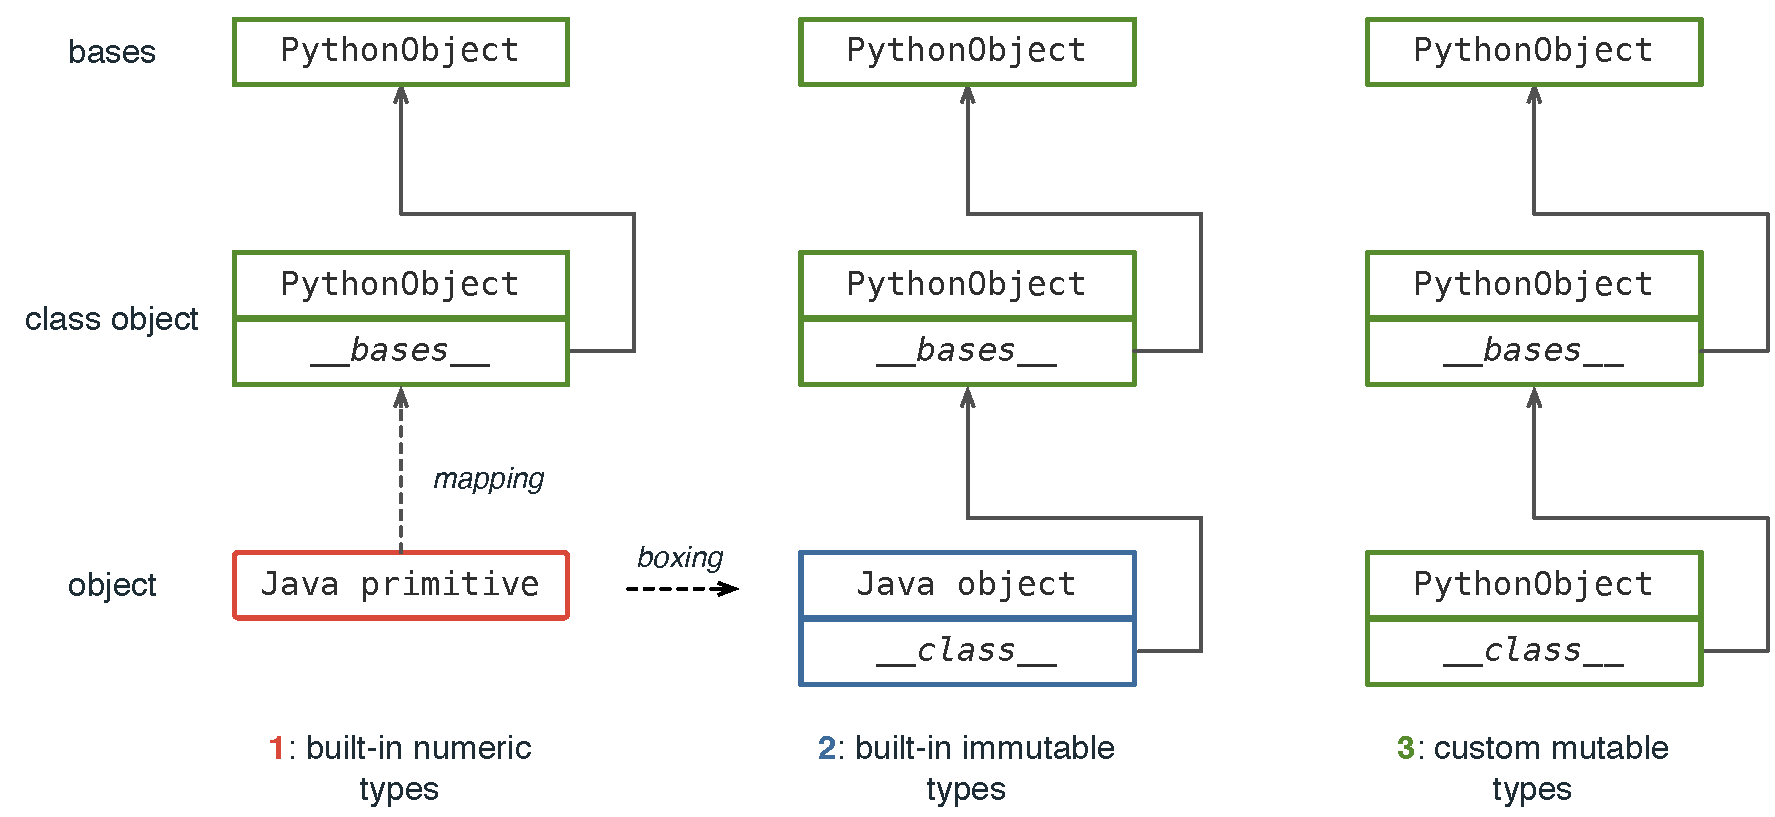
\includegraphics[scale=.54]{figures/ch5-attribute-resolutions}
\caption{Attribute resolution for different data representations}
\label{fig:ch5-attribute-resolutions}
\end{figure}

Since ZipPy uses multiple data representations to model Python objects, we also need to implement the above mentioned attribute resolution differently for each representation.
Figure~\ref{fig:ch5-attribute-resolutions} illustrates this process for the three different data representations used in ZipPy.
For simplicity, we model all class objects using a mutable \texttt{PythonObject}.
Each \texttt{PythonObject} stores the reference to the next node in the lookup chain as a dedicated field (\texttt{\_\_class\_\_} and \texttt{\_\_bases\_\_}).
This choice makes the type hierarchy of mutable objects consistent, since every node on the lookup chain is a \texttt{PythonObject}.
Similarly, built-in types modeled using immutable Java objects connect to the rest of the lookup chain also use a reference stored in a dedicated field.
For unboxed built-in types, we uses a preprocessed mapping table to associate the Java class of the primitive type to the class object representing its Python type.
For instance, we model a Python integer, which is an instance of the Python \texttt{int} class, using a Java primitive \texttt{int}.
However, we model the Python \texttt{int} class object itself, which is an instance of the class \texttt{type}, using a mutable Java object.
The mapping table maps the Java class of primitive \texttt{int} to the Python \texttt{int} class object, and thus completes the entire lookup chain for unboxed built-in types.

\subsection{Modeling Custom Mutable Types}
\label{sec:ch5-custom-mutable-types}

\begin{figure}
\centering
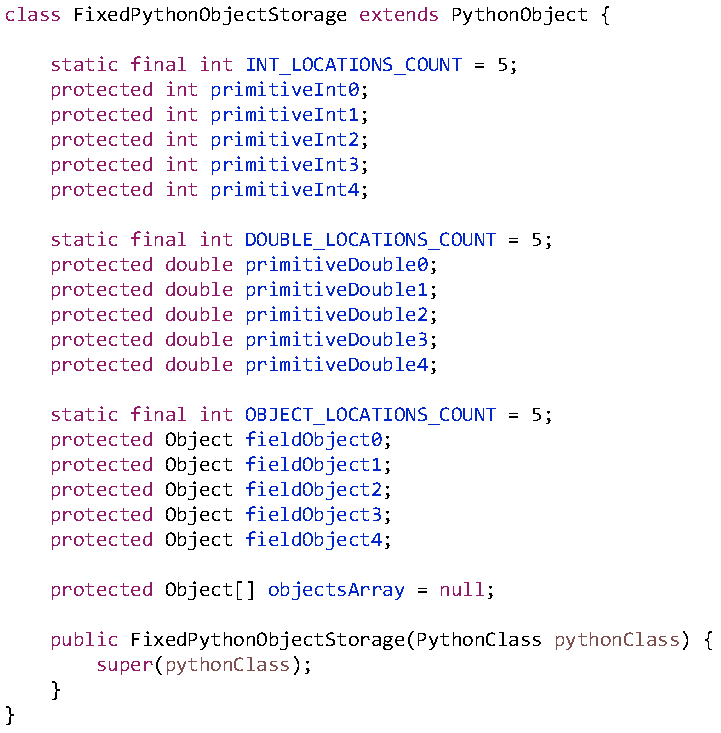
\includegraphics[scale=1.]{figures/ch5-fixed-python-object-code}
\caption{The implementation of \texttt{PythonObject}}
\label{ch5-fixed-python-object-code}
\end{figure}

\begin{figure}
\centering
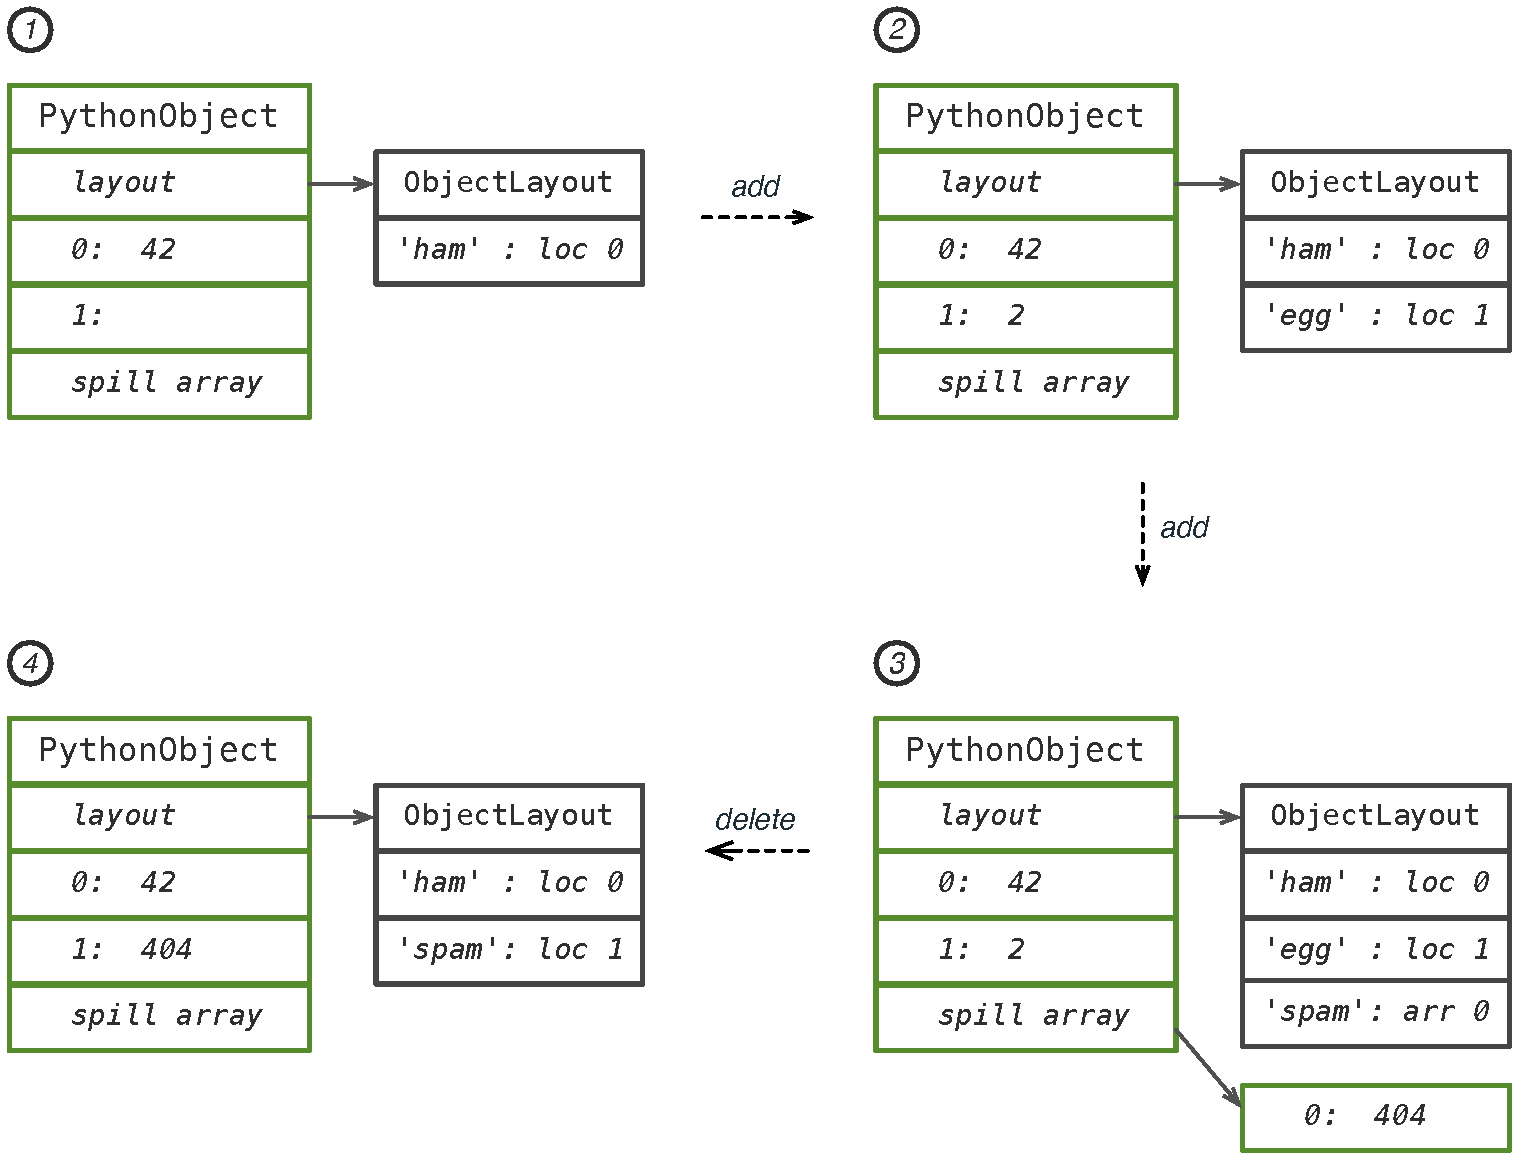
\includegraphics[scale=.6]{figures/ch5-mutable-object-layout-change}
\caption{Mutable object layout}
\label{ch5-mutable-object-layout-change}
\end{figure}

Python allows programmers to add, modify or delete attributes on an object during the execution of the program.
On the other hand, a Java object is fixed.
You can modify the value of a field, but cannot resize or change the layout of an object.
We support this dynamic feature of Python by implementing each Python object using a combination of a fixed \texttt{PythonObject} and a re-sizable object layout.

Figure~\ref{ch5-fixed-python-object-code} shows an implementation of \texttt{PythonObject} in ZipPy.
Each \texttt{PythonObject} has a fixed number of fields of both primitive and reference types to accommodate its attributes.
Each field on the object is a \emph{location}.
The object stores each of its attribute on a dedicated \emph{location}.
ZipPy tries to store an unboxed attribute in an unboxed location to avoid the overhead of boxing.
For instance, it tries to store a Java \texttt{int} in an \texttt{int} field when possible.
If all \texttt{int} fields are taken, it tries to stores the attribute in an \emph{boxed} location or an object field.
If no in-object location is available anymore (taken by other attributes), ZipPy will spill the incoming attribute to be stored in the additional object array (field \texttt{objectArray} in Figure~\ref{ch5-fixed-python-object-code}).
The additional object array gives the fixed \texttt{PythonObject} the ability to store more attributes than its own capacity by paying the price of another level of direction and possibly auto-boxing.

An object layout attached to a \texttt{PythonObject} keeps track of the list of attributes stored on the object as well as the location of each attribute.
It is essentially a table that maps the symbol of an attribute to its location.
The table records modifications made dynamically to the attributes of the object.
Figure~\ref{ch5-mutable-object-layout-change} illustrates how this process works by using a hypothetical Python object.
The layout of the shown object goes through the following stages:

\begin{enumerate}

\item The object initially has one attribute \textsf{ham} stored in location $0$ with the value $42$.

\item After adding the attribute \textsf{egg}, the object now has both \textsf{ham} and \textsf{egg} stored in location $0$ and $1$ respectively.

\item Since both in-object locations are taken, the object stores the new attribute \textsf{spam} in the spill array at the index $0$.
The rest of the layout remain unchanged.

\item The deletion of \textsf{egg} frees location $1$ on the object.
The object reassigns the newly available in-object location to \textsf{spam} to make sure that location assignments are optimal.
It also update the layout table to reflect the new changes.

\end{enumerate}

We simplified the structure of the Python object shown in Figure~\ref{ch5-mutable-object-layout-change} for brevity.
The actual algorithm for a layout update is more complicated.
Adding or deleting an attribute triggers a layout update.
The layout update tries to stores as many unboxed attributes in an unboxed location as possible.
The spill array allocation is lazy so that we only allocate the array when necessary.
During the layout update, ZipPy calculates the size of the additional spill array needed to accommodate all the attributes.
If it requires a spill array, we conservatively allocate an array that is just enough to store all the attributes.

The type of an attribute can change at runtime.
A type change also triggers a layout update.
Our current solution is to assign a location that matches the most general type of an attribute.
Once an unboxed attribute becomes boxed, we always assign a boxed location for this attribute in the future.

Our approach uses \texttt{PythonObject}s simply as a physical storage for the attributes of a Python object.
We detach the layout description of the Python object from its storage component, which gives us the freedom to customize the behavior of attribute accesses in ZipPy without being restricted by Java's own object model.
Since we model class objects in the same way as regular objects in Python, they enjoy the same potential performance benefit achieved by this design.

\subsection{Inline Caching for Attribute Accesses}

As explained in Section~\ref{sec:ch5-custom-mutable-types}, the layout table stores the location of each object attribute.
Access an attribute requires looking up its location information from the layout table and then performing a memory operation that reads from or writes to the obtained memory location.
Since we implement the layout table using a hash map, the cost of accessing the table is as expensive as attribute accesses on a hash map based object.
However, ZipPy optimizes attribute accesses by caching attribute locations after a full layout table lookup.
This technique, inspired by previous research on virtual machines~\cite{Deutsch1984, holzle1991, Brunthaler2010inca}, amortizes the cost of accesses to the same attribute on the object of the same type.

\subsubsection{Attribute Access Dispatch Chain}
\label{sec:ch5-attribute-access-dispatch-chain}

\begin{figure}
\centering
\subfigure[Structure of \texttt{GetAttributeNode}]{
	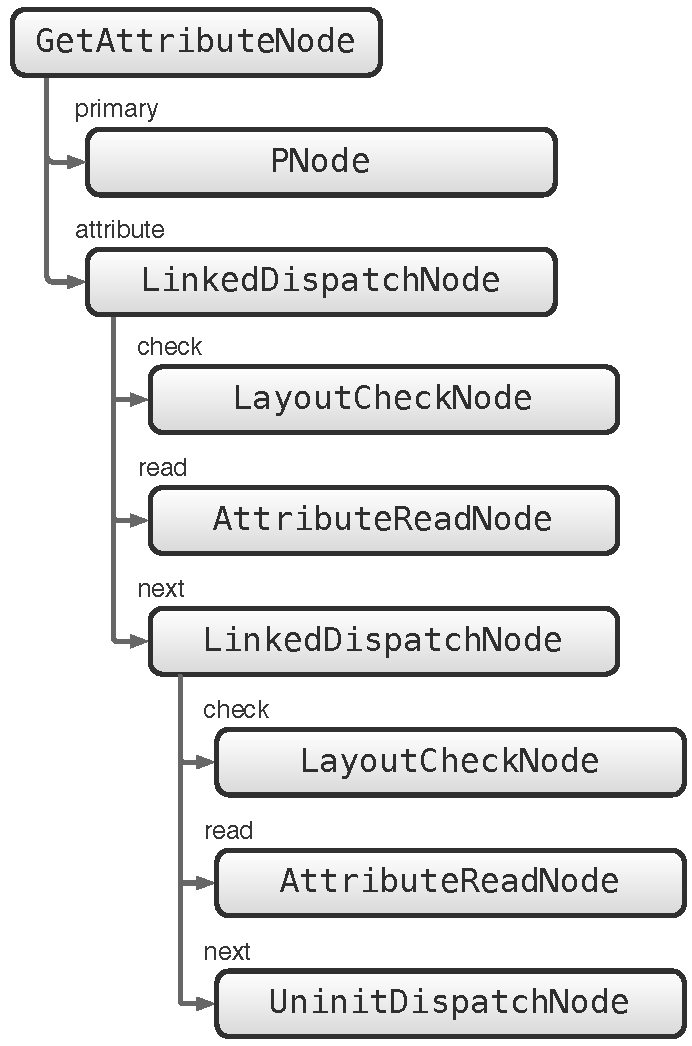
\includegraphics[scale=.55]{figures/ch5-get-attribute-node}
	\label{fig:ch5-get-attribute-node}
}
\subfigure[Structure of \texttt{SetAttributeNode}]{
	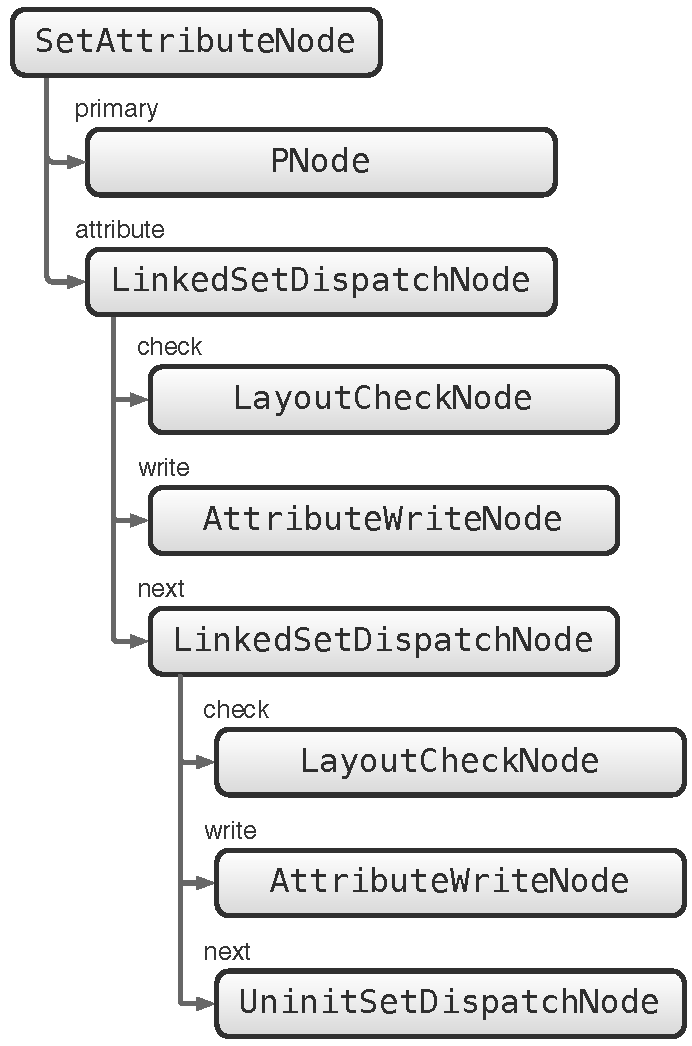
\includegraphics[scale=.55]{figures/ch5-set-attribute-node}
	\label{fig:ch5-set-attribute-node}
}
\caption{Attribute access dispatch chain}
\label{fig:ch5-attribute-access-dispatch-chain}
\end{figure}

Like the other operation, we model attribute accesses using AST nodes in ZipPy.
We model an attribute read operation using a \texttt{GetAttributeNode} and write operation using a \texttt{SetAttributeNode}.
Figure~\ref{fig:ch5-attribute-access-dispatch-chain} illustrates the structure of these two nodes.
In each attribute access node, the \textsf{primary} child node represents the primary expression, the component precedes the period in Python's syntax.
The \textsf{primary} node evaluates to the Python object, on which we perform the attribute access.
The \textsf{attribute} nodes shown in both Figure~\ref{fig:ch5-get-attribute-node} and~\ref{fig:ch5-set-attribute-node} are dispatch chains that perform the actual read or write on the resolved object.

The attribute access dispatch chain is a link list of dispatch nodes.
Each dispatch node has a \textsf{next} field that points to the next dispatch node except for the last one.
The chain forms a polymorphic inline cache with each node working as an individual cache entry.
Each entry stores the object layout and the location of a previously accessed attribute.
Upon a successive access to the attribute on an object having the same layout, the matching dispatch node performs a memory access directly using the cached location.
In other words, a cache hit in the dispatch chain voids executing the slow path lookup on the object layout.

ZipPy performs an attribute access operation in a number of steps.
It first evaluates the primary object, and passes the object to the dispatch chain.
The resolved primary object travels through the dispatch chain from the top to the bottom one dispatch node after another.
Each dispatch node tests the cached object layout against the one of the incoming object.
If the test returns a match, the dispatch node performs a fast read or write on the object and returns the result to the parent node if necessary.
Otherwise, execution falls to the next dispatch node on the chain until a cache hit occurs.
If no cache hit happened, the primary object reaches the uninitialized dispatch node at the end of the chain.
The uninitialized dispatch node, in this case, performs a full attribute access on the primary object including a lookup on its layout table.
Additionally, it also constructs a new cached dispatch node and inserts the new node between the uninitialized dispatch node and its predecessor.
The added entry increases the depth of the inline cache as well as the chance of a cache hit in the future.
However, if the cache depth reaches a certain threshold, ZipPy rewrites the entire dispatch chain to a single generic dispatch node that always perform a slow path lookup.

Each cache entry in the dispatch chain consists of a cluster of nodes coordinated by the dispatch node.
Besides the \textsf{next} field pointing to the next node, each dispatch node has a \texttt{LayoutCheckNode} as well as a \texttt{AttributeReadNode} or \texttt{AttributeWriteNode} (Figure~\ref{fig:ch5-attribute-access-dispatch-chain}).
The \textsf{check} node stores the cached object layout and performs the layout test.
The \textsf{read} or \textsf{write} node stores the cached attribute location and performs the actual read or write on the primary object.
When a layout update happens, ZipPy creates a new layout instance for the associated Python object.
ZipPy also signals the old layout as invalid, since it does not describe a valid layout for the associated object anymore.
Therefore, when performing a layout test the \texttt{LayoutCheckNode} also checks the validity of the cached layout.
If the cached layout become invalid, it throws an exception back to the parent node.
ZipPy handles the exception by remove the invalid cache entry from the dispatch chain.

\subsubsection{Dispatch Node Transformation}

\begin{figure}
\centering
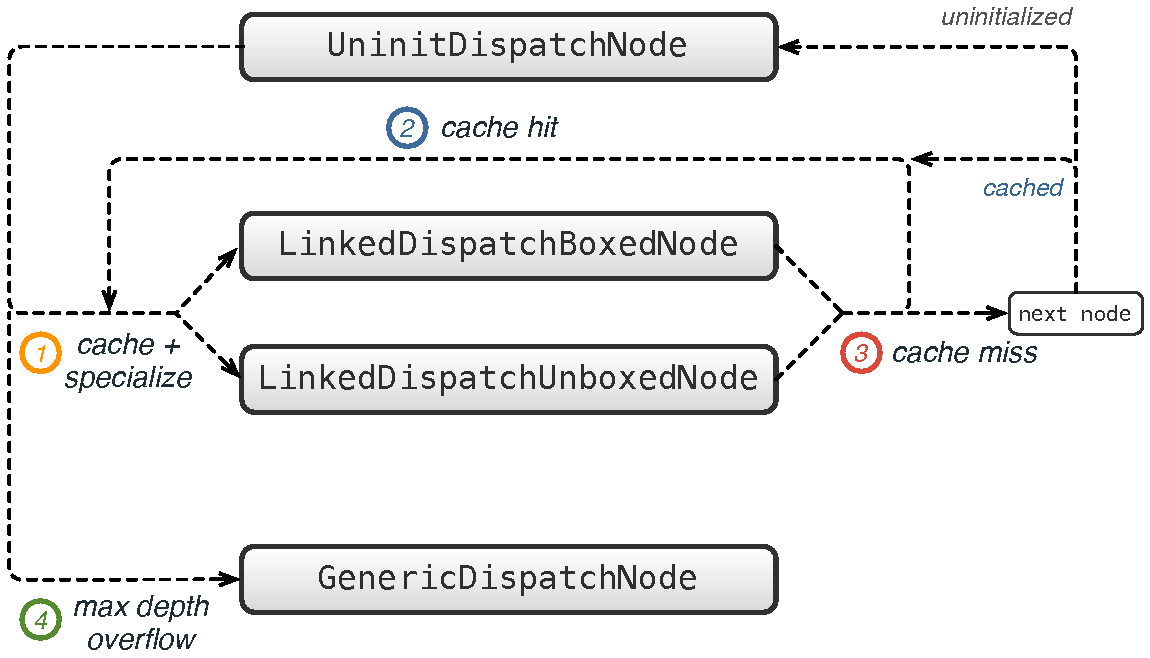
\includegraphics[scale=.65]{figures/ch5-attribute-dispatch-transformation}
\caption{The transformation of a get attribute dispatch node}
\label{fig:ch5-attribute-dispatch-transformation}
\end{figure}

The above mentioned attribute access dispatch chain initially starts with a single uninitialized dispatch node.
It expands into a chain linking a number of \texttt{LinkedDispatchNode} during execution.
If the depth of the chain overflows a given limit, the entire chain transforms to a \texttt{GenericDispatchNode}.
Figure~\ref{fig:ch5-attribute-dispatch-transformation} further illustrates this transformation.
The descriptions of the transformation rules depicted in the Figure are as follows:

\begin{enumerate}

\item Upon a successful specialization, the uninitialized dispatch node produces a specialized dispatch node that caches the layout of the primary object and the location of the attribute being accessed.
Depending on the data representation of the primary object, it chooses the \texttt{LinkedDispatchUnboxNode} as the transformation target to avoid auto-boxing.
A \texttt{LinkedDispatchUnboxNode} stores the Java class of the \emph{unboxed} object.

\item A \texttt{LinkedDispatchBoxedNode} performs the layout test through an identify check between the cached layout and the layout of the incoming primary object.
A layout test on a \texttt{LinkedDispatchUnboxedNode} compares the cached Java class to that of the primary object.
If the layout test returns a match, the cached dispatch node remains unchanged.
Note that in an attribute read operation, as explained in Section~\ref{sec:ch5-attribute-resolution}, the resolved attribute may not be stored on the primary object itself.
In fact, the actual owner can be any object on the attribute resolution chain of the primary object.
In this case, the cached dispatch node needs to conservatively cache all the layout of the objects on the attribute resolution chain from the primary object itself up to the owner of the resolved attribute.
In the layout test, the dispatch node needs to perform a series of checks to ensure the validity of the cache layouts.

\item If the layout test returns a miss match or a cache miss occurs, the cached dispatch node redirects execution to the next node on the dispatch chain.
The same rules apply to the transformation of the next dispatch node.
In addition, if the cached layout become invalid, ZipPy removes the dispatch node from the chain.

\item If the execution of an attribute access dispatch reaches an uninitialized dispatch node and the depth of the chain has reached a certain threshold,
the dispatch node replaces the entire dispatch chain with a \texttt{GenericDispatchNode}.
A \texttt{GenericDispatchNode} is stable meaning that it always perform a slow path attribute lookup and does not re-specialize to other nodes.

\end{enumerate}

The deeper the dispatch chain the more step it takes to reach the bottom portion of the chain.
The cost of hitting a cache entry located close to the bottom of the chain grows with the depth of the chain.
Thus, it is not cost effective to grow the dispatch chain indefinitely.
On the other hand, for a program location exhibits a high degree of polymorphism or also referred as a megamorphic dispatch site,
optimizing for just a few number of cases only affects a limited fraction of the overall execution occurred at this program location.
An optimization strategy like inline caching is unlikely to have an substantial performance impact in this case.
In summary, for a megamorphic dispatch site using a generic dispatch node is simpler and as efficient as forming a deep dispatch chain.

\section{Call Site Modeling}

Calls are common in Python programs.
In general you can call any \emph{callable} object in Python.
However, there are different ways to make a call in Python.
In different contexts the semantics of a call in Python also differs, which makes it surprisingly difficult to model various types of call sites in an efficient way.

\subsection{Call Site Structures in Python}
\label{sec:ch5-structure-of-call-sites}

\begin{figure}
\centering
\subfigure[Simple call site]{
	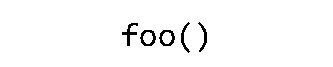
\includegraphics[scale=.9]{figures/ch5-call-site-simple-code}
	\label{fig:ch5-call-site-simple-code}
}
\subfigure[Attribute call site]{
	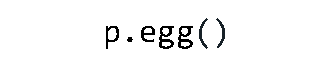
\includegraphics[scale=.9]{figures/ch5-call-site-attribute-code}
	\label{fig:ch5-call-site-attribute-code}
}
\caption{Two types of calls in Python}
\label{fig:ch5-call-site-synteax-code}
\end{figure}

Figure~\ref{fig:ch5-call-site-simple-code} shows the basic syntax of a call in Python.
It is simple enough for us to explain the basic steps of making a call in Python without getting into more complicated details.
The execution of the call shown in the Figure involves the following steps.
First, the program needs to lookup the symbol \texttt{ham} from the current scope or its enclosing scope with respect to Python's scoping rules.
After resolving the callee, the program then checks the type of the callee to determine the eligibility of such call.
Lastly, the actual call takes place using a calling convention that matches the callee type.
The Python interpreter handles argument passing differently for different callee types.
For instance, a constructor call, a call to a Python class object, creates an instance of the Python class.
In a constructor call, the interpreter creates an empty Python object and passes it to the callee as the first argument.

The call site shown in Figure~\ref{fig:ch5-call-site-simple-code} is in its simplest form.
We refer it as a \emph{simple call site}.
The callee resolution for the call shown in Figure~\ref{fig:ch5-call-site-attribute-code} involves an attribute access on the Python object \texttt{p}.
Therefore, we refer this type of call site as \emph{attribute call sites}.
The primary object, however, can be any namespace backed by a Python object such as a regular object, a class object or a module.
Note that, in a simple call site, the callee resolution might involve an attributing access as well depending on the type of the surrounding scope where the call takes place.
For example, if \texttt{ham} is a global variable, the look up of \texttt{ham} includes an implicit attribute access on the global scope object or the Python module.
Similarly, in a class scope, a simple call to an existing class attribute also involves an implicit attribute look up on the enclosing class object.
% say something about motivates the structure of the AST
The same syntax implies different semantics and ways to make the actual call at runtime.
To cover different variations, we decompose a call site in ZipPy into multiple of components or nodes and assemble them in various ways to serve our needs.
This way allows us to apply specializations on each component separately to optimize calls in Python programs.

\subsubsection{The AST of Call Sites}

\begin{figure}
\centering
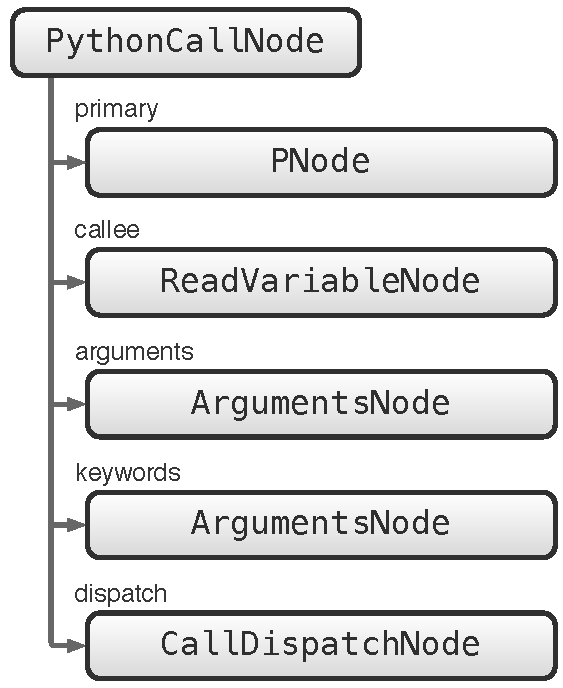
\includegraphics[scale=.5]{figures/ch5-python-call-node-basic}
\caption{The structure of a \texttt{PythonCallNode}}
\label{fig:ch5-python-call-node-basic}
\end{figure}

Figure~\ref{fig:ch5-python-call-node-basic} illustrates the basic structure of a call node in ZipPy.
A \texttt{PythonCallNode} employees five child nodes representing five components of the call site.
Each child node can further expand into its own sub tree depending on its complexity.
A call node performs a Python call incorporating its child nodes in the following steps:

\begin{enumerate}

\item The primary node evaluates the primary object of the call.
If the primary component is missing, the primary node returns the constant Python \texttt{None} object.

\item The callee node resolves the actual callee object using the previously resolved primary object if necessary.
If the callee resolution does not involve an attribute access, it ignores the primary object.

\item The arguments node evaluates all the arguments, and returns them to the call node as a Java array.

\item The keywords node evaluates all the keyword arguments, and returns them to the call node in an Java array.

\item The \texttt{PythonCallNode} passes the evaluated primary object, callee, arguments array and keyword arguments array to the dispatch node.
The dispatch node performs the actual call using an inline caching inspired dispatch chain scheme~\cite{Deutsch1984, holzle1991}, and passes all the arguments to the AST of the callee.
We will explain the call dispatch nodes in more detail in Section~\ref{sec:ch5-call-site-caching-and-inlining}.

\end{enumerate}

Note that some components like the primary or keyword arguments are not always present.
In case that an optional component is missing, we still model it as a dummy node that returns a \texttt{None} or an empty Java array to make it consistent for all call nodes.
The \texttt{PythonCallNode} organizes different components of the call site and handles transformations like type specialization and deoptimization at runtime.

\subsection{Call Node Specializations}

Similar to other operations in ZipPy, we applies type specializations to call nodes against the type of the callee through node rewriting.
It initially constructs a call node using the uninitialized version (\texttt{UninitCallNode} in Figure~\ref{fig:ch5-call-node-specialization-simple}).
Upon the first execution of the call, the uninitialized call node executes a slow path to resolve the primary object and callee.
At the same time, it rewrites itself to a derivative version that is tailored to the resolved primary and callee.
Not only that the call node specializes itself, it also applies type specializations to its child nodes during the rewriting process.
In this Section, we explain how ZipPy applies call node specializations for different call sites and callee types.

\subsubsection{Specialization for Simple Call Sites}

\begin{figure}
\centering
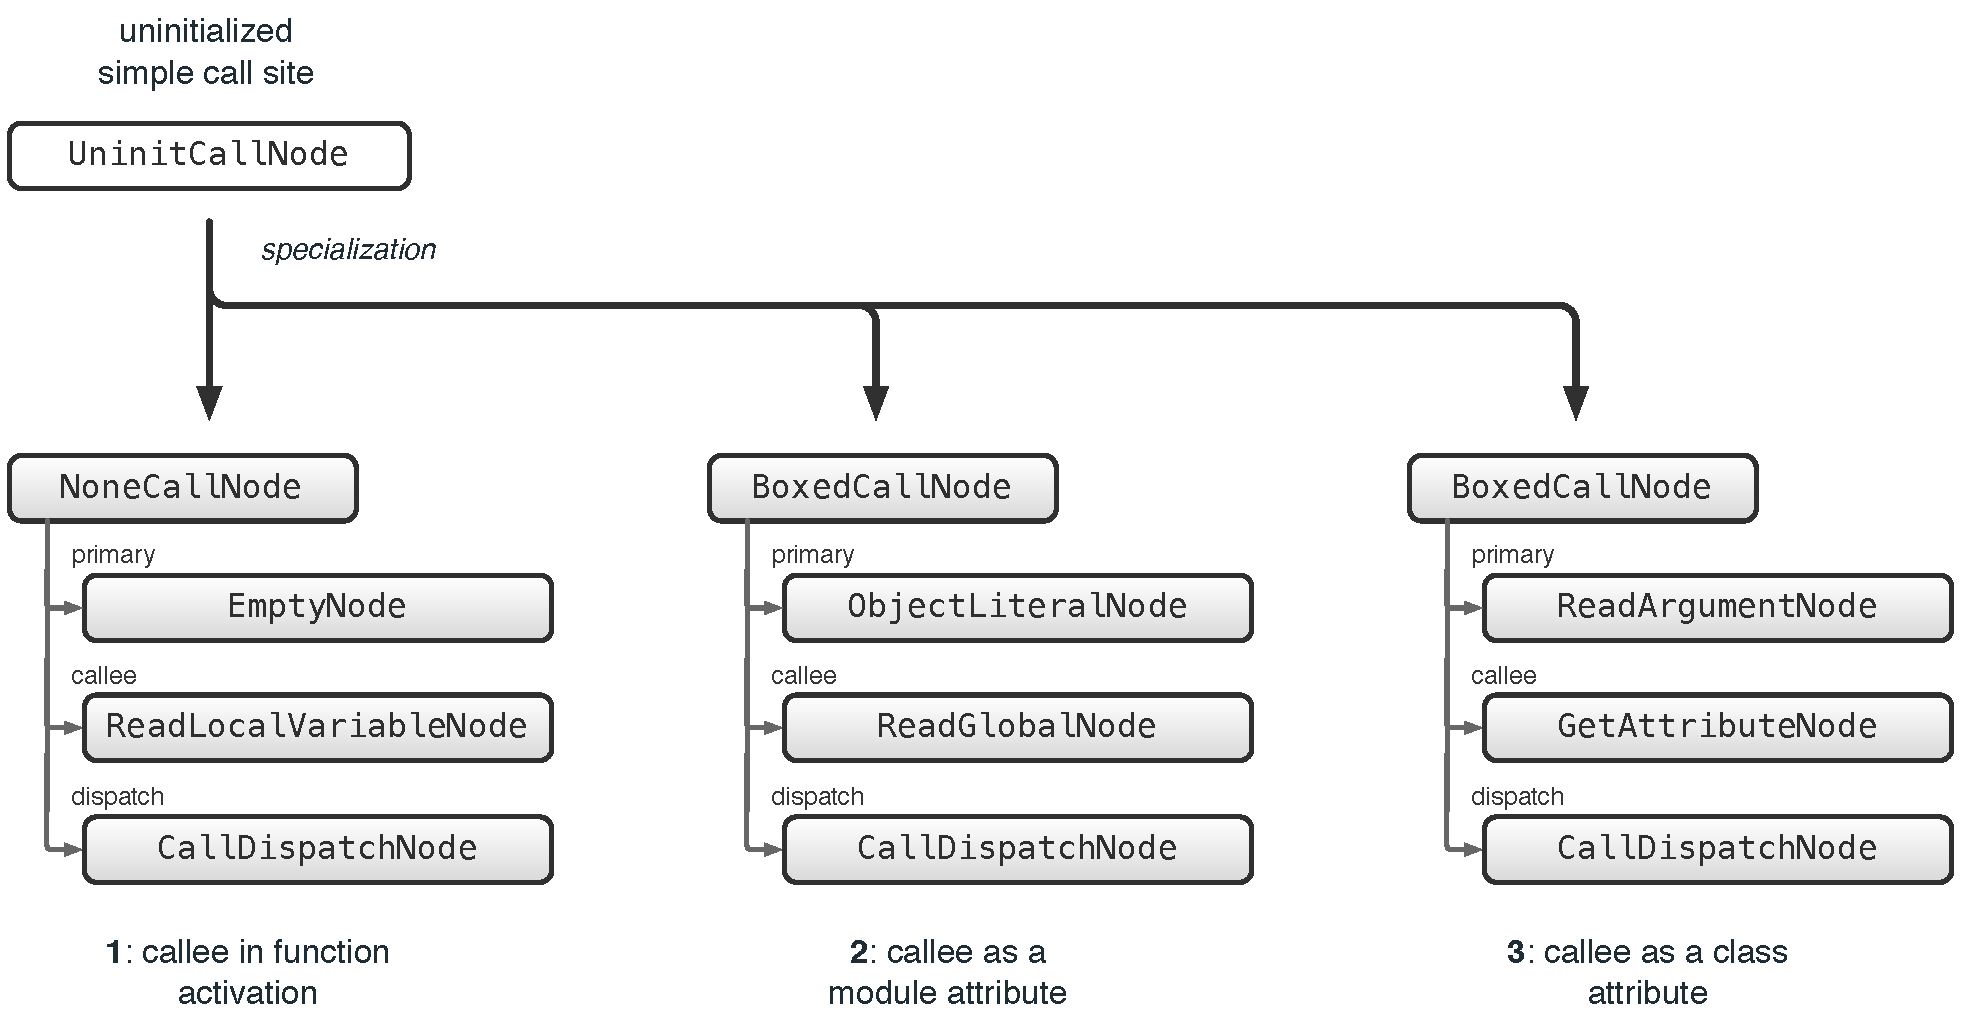
\includegraphics[scale=.5]{figures/ch5-call-node-specialization-simple}
\caption{Call node specializations for a simple call site}
\label{fig:ch5-call-node-specialization-simple}
\end{figure}

As explained in Section~\ref{sec:ch5-structure-of-call-sites}, the callee resolution of a simple call site (Figure~\ref{fig:ch5-call-site-simple-code}) depends on the type of the namespace to which the callee belongs.
Therefore, the specialization of a simple call site needs to cover different resolution cases.
Figure~\ref{fig:ch5-call-node-specialization-simple} illustrates various call node transformations of a simple call site.
The description of the three different specialization cases shown in the Figure is as follows:

\begin{enumerate}

\item \textbf{Callee in function activation}
The call takes place in a function scope.
The resolved callee is a variable of the function's lexical scope or its enclosing scope.
The primary object does not exist or is \texttt{None} in this case.
Therefore, the primary node is an \texttt{EmptyNode} that returns an \texttt{None}.
The callee nodes retrieve the callee object from the function's activation or the frame object as discussed in Chapter~\ref{sec:ch4-frame-and-control}.
Although type specialization is also applicable to the \texttt{ReadLocalVariableNode}, given that the callee is guarantee to be a boxed object, type specialization in this case has limited benefit.
However, Truffle is still able to optimize frame accesses by eliminating heap allocation of the frame object when applicable.

\item \textbf{Callee as a module attribute}
The resolved callee is an attribute of a module, e.g., the global scope of the current module or the built-in module.
The retrieval of the callee in this case involves an implicit attribute referencing on the primary module object.
Since the primary object is boxed, ZipPy specializes the call node to a \texttt{BoxedCallNode}.
The primary node is a wrapper node that holds a reference to the current module object.
The callee node reads the callee attribute from the module object returned by the primary node.
The \texttt{ReadGlobalNode} accesses the built-in module if it failed to resolve it from the global scope module.
Upon a successful resolution of the callee object, the \texttt{ReadGlobalNode} caches the actual primary object.
For instance, if the resolved callee object is an attribute of the built-in object, the node caches the built-in object instead of the current module.
Caching speedups subsequent attribute accesses by accessing the cached object directly as long as the attributes of the object remain unchanged.

\item \textbf{Callee as a class attribute}
The call takes place in a class scope.
The resolved callee is an existing class attribute of the enclosing scope.
Class definition works as a special function in Python.
The evaluation of the class definition statement is essentially a call to the special function.
The interpreter passes an empty class object as the first argument to the function, and the class definition function populates the class object with attributes like functions.
The call to the class definition function returns the created class object containing attributes specified by in the class definition.
To access an existing attribute of the defining class, we need to first retrieve the defining class object.
The \texttt{ReadArgumentNode} does so by reading the argument array passed by the caller of the class definition.
the callee node then reads the callee attribute from the primary class object.
The \texttt{GetAttributeNode} also enjoys type specialization and caching on its own, which we will discuss more in Section~\ref{sec:ch5-object-module}.

\end{enumerate}

The call node specializations illustrated in Figure~\ref{fig:ch5-call-node-specialization-simple} are based on the resolution of the primary object and callee.
We simplified the Figure by not including the arguments node and the keyword arguments node, since their specializations are orthogonal to callee resolutions.

\subsubsection{Specialization for Attribute Call Sites}

\begin{figure}
\centering
\subfigure[Boxed primary]{
	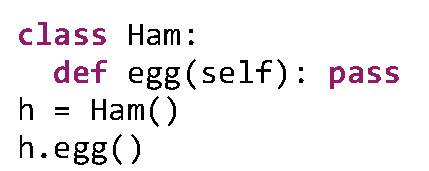
\includegraphics[scale=.7]{figures/ch5-attribute-call-site-boxed-code}
	\label{fig:ch5-attribute-call-site-boxed-code}
}
\subfigure[Unboxed primary]{
	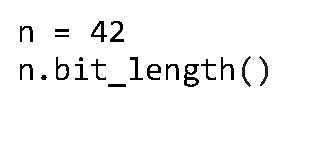
\includegraphics[scale=.7]{figures/ch5-attribute-call-site-unboxed-code}
	\label{fig:ch5-attribute-call-site-unboxed-code}
}
\caption{Attribute call sites with different primary object representations}
\label{fig:ch5-attribute-call-site-boxed-unboxed-code}
\end{figure}

In Section~\ref{sec:ch5-object-module} we discussed that ZipPy models Python objects using multiple data representations to make arithmetics and object operations more efficient.
As a consequence, attribute accesses on objects modeled using different representations are also different.
Figure~\ref{fig:ch5-attribute-call-site-boxed-unboxed-code} shows two examples of attribute call sites.
The primary object in the left example --- \texttt{h} --- is a custom Python object (Figure~\ref{fig:ch5-attribute-call-site-boxed-code}),
whereas the primary object \texttt{n} in the right one (Figure~\ref{fig:ch5-attribute-call-site-unboxed-code}) is a built-in integer.
The callee resolutions in these two cases are different.

\begin{figure}
\centering
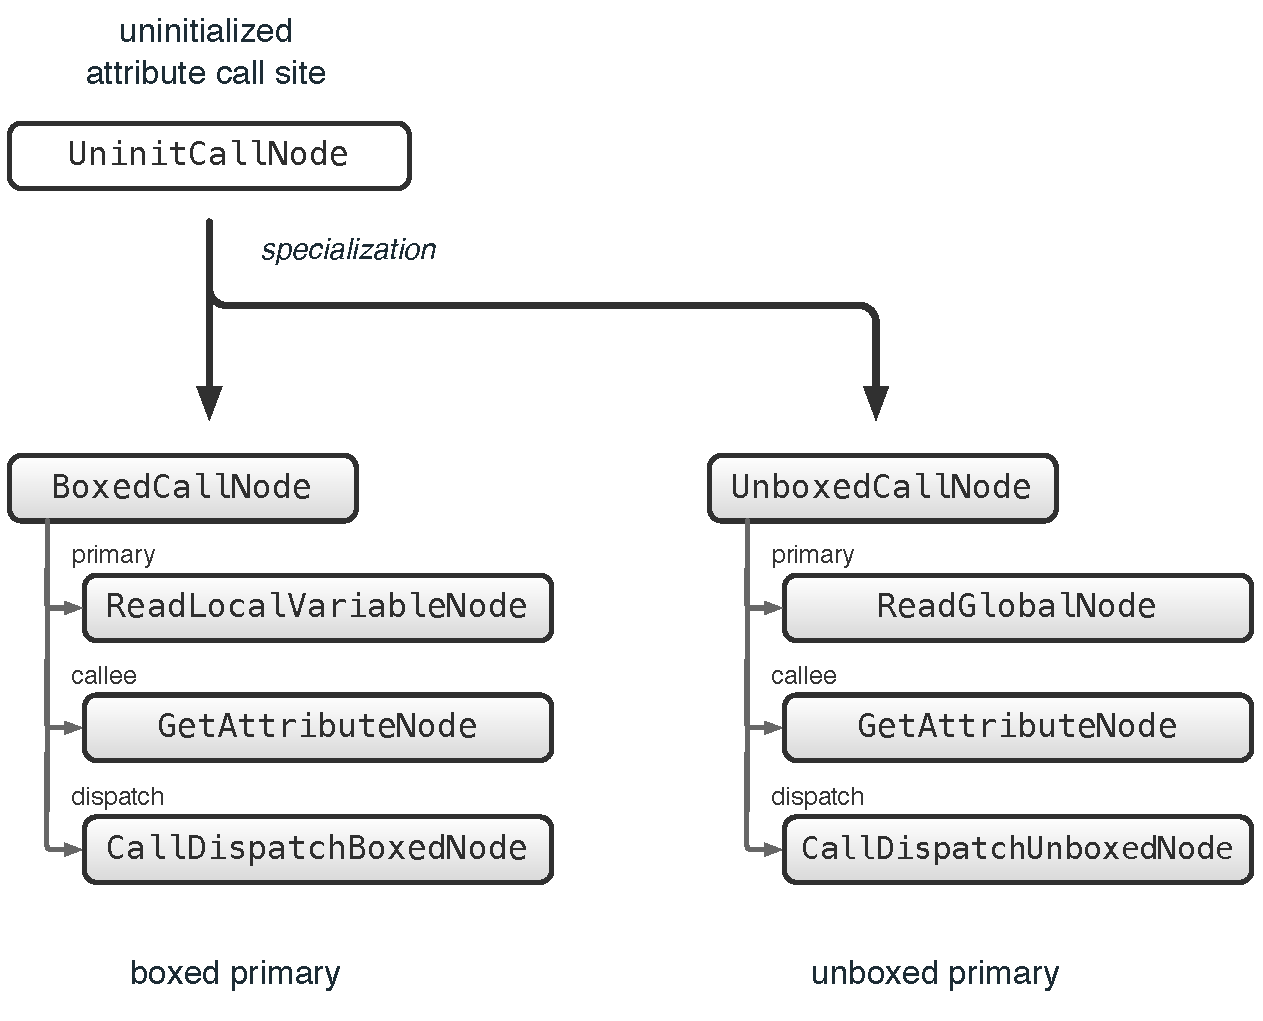
\includegraphics[scale=.5]{figures/ch5-call-node-specialization-attribute}
\caption{Call node specializations for an attribute call site}
\label{fig:ch5-call-node-specialization-attribute}
\end{figure}

Figure~\ref{fig:ch5-call-node-specialization-attribute} illustrates the specializations we implemented in ZipPy to handle both boxed and unboxed primary types in an attribute call site.
A \texttt{BoxedCallNode} expects a mutable Python object as the primary and walks its attribute resolution chain upward to resolve the callee.
A \texttt{UnboxedCallNode} on the other hand expects an unboxed primary object.
It obtains the primary's class object through the mapping table explained in Section~\ref{sec:ch5-attribute-resolution} to access the primary's attribute resolution chain.

In Python, an attribute reference that looks up a \texttt{PyFunction} object creates a \texttt{PyMethod} that wraps both the primary and the \texttt{PyFunction} objects.
If the \texttt{PyMethod} is invoked at another program location, it passes the stored primary object to the actual callee as the first argument.
The \texttt{PyMethod} creation guarantees the data binding between the primary and its function attribute.
However, in most cases, the allocation of the \texttt{PyMethod} object is unnecessary.
In an attribute call site, the resolved callee is invoked right away and does not escape the program location where it is referenced.
Therefore, there is no need to create the wrapper for it.
By applying specialization for attribute call sites in ZipPy we eliminate the creation of \texttt{PyMethod} objects in most cases.

\subsubsection{Specialization for Special Method Call Sites}

\begin{figure}
\centering
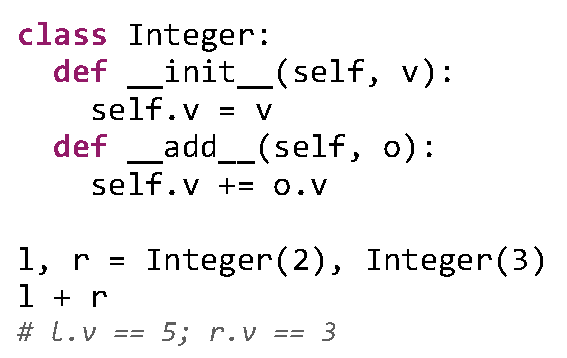
\includegraphics[scale=.7]{figures/ch5-special-method-add-code}
\caption{Operator overloading by overwriting special method}
\label{fig:ch5-special-method-add-code}
\end{figure}

Python support operator overloading by allowing user defined classes to overwrite a set of special methods.
Those special methods all have underscores in their names.
Figure~\ref{fig:ch5-special-method-add-code} gives an example of overloading the add operation.
By overwriting the \texttt{\_\_add\_\_} method, the shown program redefines the behavior of the add operation on the custom type \texttt{Integer}.
Therefore, the add operation on the last line of the program shown in Figure~\ref{fig:ch5-special-method-add-code} performs an in-place update on the object \texttt{l}.
In the end, the values of the attribute \texttt{v} on the object \texttt{l} and \texttt{r} equal to $5$ and $3$ respectively.

\begin{figure}
\centering
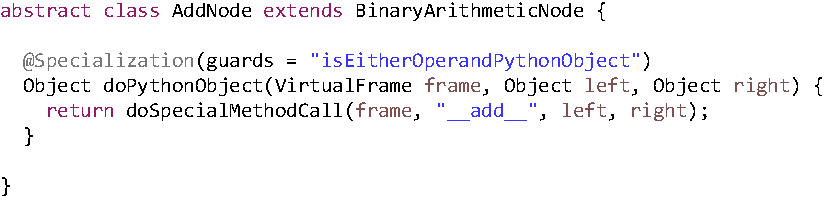
\includegraphics[scale=1.]{figures/ch5-add-node-special-method-code}
\caption{\texttt{AddNode} specialization for special method overwriting}
\label{fig:ch5-add-node-special-method-code}
\end{figure}

To support special method overwriting in ZipPy, we applied additional specializations to the operation nodes that support overloading.
As an example, Figure~\ref{fig:ch5-add-node-special-method-code} shows such a specialization we added to the \texttt{AddNode} in ZipPy.
Add is a binary operation.
So an \texttt{AddNode} in ZipPy specializes against the types of the two operands.
If either of the operand is a boxed Python object or of type \texttt{PythonObject} we specialize this add operation as a special method call.
The call to \texttt{doSpecialMethodCall} shown in the Figure tries to lookup the special method \texttt{\_\_add\_\_} from the operands and invoke it.
At the same time, it also constructs a call dispatch chain that performs the actual invocation and attaches the chain to the add node.

\begin{figure}
\centering
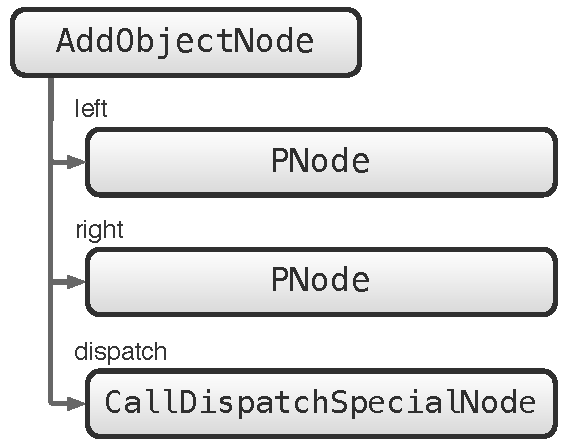
\includegraphics[scale=.5]{figures/ch5-add-node-with-special-dispatch}
\caption{\texttt{AddNode} specialized for special method dispatch}
\label{fig:ch5-add-node-with-special-dispatch}
\end{figure}

Figure~\ref{fig:ch5-add-node-with-special-dispatch} illustrates the structure of an add node after successfully specialized for a special method call.
First, ZipPy specializes the add node itself to an \texttt{AddObjectNode} based on the operand types.
The left and right children of the add node can be nodes of any time.
We simply mark them as \texttt{PNode}s here to show their existences.
More interestingly, a call dispatch chain represented by the \texttt{CallDispatchSpecialNode} appears as a child of the add node.
A call dispatch chain is similar to an attribute access dispatch chain.
It forms an inline cache for calls, which we will explain in more detail in Section~\ref{sec:ch5-call-site-caching-and-inlining}.
When executing a subsequent call to the special method, the add node first evaluates the operands and passes them to the call dispatch chain.
The dispatch chain performs the actual call and passes the two operands as arguments to the callee.

\subsection{Call Site Dispatch and Inlining}
\label{sec:ch5-call-site-caching-and-inlining}

\begin{figure}
\centering
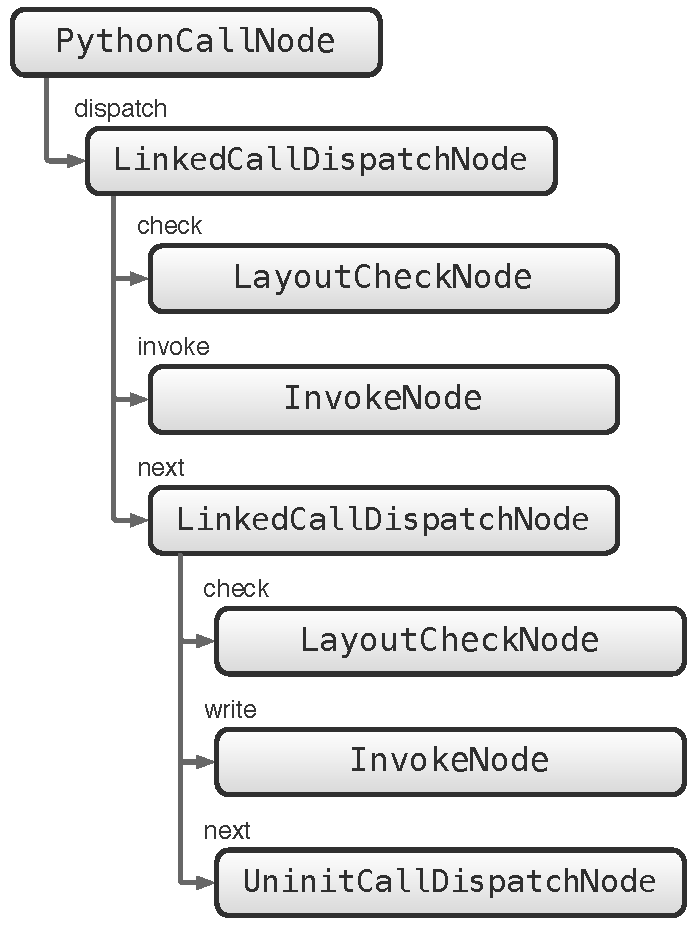
\includegraphics[scale=.5]{figures/ch5-call-dispatch-chain}
\caption{Call dispatch chain}
\label{fig:ch5-call-dispatch-chain}
\end{figure}

The most effective way to optimize a call is to avoid the call altogether.
In other words, inlining helps to eliminate the overhead incurred by calls.
However, the dynamic features of Python makes call inlining more challenging to implement.
Any callable is a first class object stored as an attribute of another object or namespace.
The value of a symbol in a namespace could change from a callable to a non-callable or a different callable object at runtime.
Due to the dynamic nature of Python, the callee resolution of a procedure call needs to happens just-in-time of the call.
A subsequent call performed at the same location does not guarantee to call the same target.

To overcome this challenge we use call dispatch chains similar to the one described in Section~\ref{sec:ch5-attribute-access-dispatch-chain} to optimize and inline calls in ZipPy.
A call dispatch chain is a chain of dispatch nodes that work as a polymorphic inline cache.
Each cache entry on the chain caches the layout of the primary object and the resolved callee of a previous call at the same call site.
Figure~\ref{fig:ch5-call-dispatch-chain} shows the components of the call dispatch chain in more detail.
Each \texttt{LinkedCallDispatchNode} represents a single cache entry.
The check node of the entry layout of a previous primary object and performs a layout test to determine a cache hit.
The invoke node stores the cached call target and call the AST of the callee.
A call dispatch chain goes through the same transformation process as an attribute dispatch chain, which starts with an uninitialized version and later on expands into a number linked dispatch nodes.
If the depth of the chain grows over threshold, the entire chain rewrites itself with a generic dispatch node.

As an AST interpreter, all Python functions are ASTs in ZipPy.
Inlining a function call is essentially stitching the AST of the callee to that of the caller at the node that represents the call site.
Truffle runtime handles the actual inlining and possibly cloning the callee AST automatically during execution.
It does so through the \texttt{InvokeNode} interface shown in Figure~\ref{fig:ch5-call-dispatch-chain}.
The \texttt{InvokeNode} stores the AST of the resolved callee and passes the arguments to the callee AST in a call.
Truffle runtime profiles the hotness of each call in the \texttt{InvokeNode} and performs call inlining by rewriting the \texttt{InvokeNode}.
Some times different call sites pass arguments of different types to the same callee.
This difference in type causes the callee AST to specialize for multiple call sites.
To void this unwanted state share between an inlined AST and the original one, Truffle clones the entire callee AST before stitches it to that of the caller.

However, Truffle's call profiling and inlining treats the entire AST as a single entity.
It does not have domain knowledge about the semantics of the guest language but only to provide building blocks that makes it easier for the guest language implementer.
To enable AST inlining, ZipPy needs to construct Python call sites using \texttt{InvokeNode}s in the way that we have described above.
Alternatively, we could handle AST inlining complete by ourselves.
From a software engineering perspective, however, this is a less desirable solution, since offloading it to the Truffle framework is easier to maintain in the long run.

\section{Flexible Object Storages}
\label{sec:ch5-flexible-object-storages}

As we described in Section~\ref{sec:ch5-object-module}, ZipPy uses a fixed Java object in combination with a dynamically updated layout table to model a mutable Python object.
This design is a common pattern shared by a number of Truffle based language implementations~\cite{seaton2014debugging,Grimmer+2014,Grimmer+2014TruffleC}.
For simplicity here we refer the fixed Java object as an \emph{object storage}, since it stores the attributes of a Python object.
We refer the Java class used to create object storages as a storage class in the rest of this thesis.
Although using a fixed object storage provides both performance efficiency and implementation simplicity, it is not optimal when it comes to space efficiency.

Most Python programs allocate small objects, which means that most of the object allocated at runtime only have a few number of attributes.
To ensure the performance of an attribute access we want to assign most attributes with a field location on the object storage.
But on the other hand is it impossible to predict the type of each attribute.
To increase the chance of an optimal location assignment, we need to increase the number of fields of each type on the object storage.
This size increase inevitably introduces more un-utilized memory space at runtime.
In addition, a fixed object storage is fixed.
For a Python object that has a large number of attributes it has to spill some of the attributes to the spill array.
This size limitation leads to performance overhead incurred by auto-boxing and more level of indirections.
In summary, fixed object storage is simple but has limitations when it comes to both performance and space efficiencies.

\subsection{Flexible Object Storage Generation}
\label{sec:ch5-flexible-object-storage-generation}

\begin{figure}
\centering
\subfigure[Python class \texttt{Point}]{
	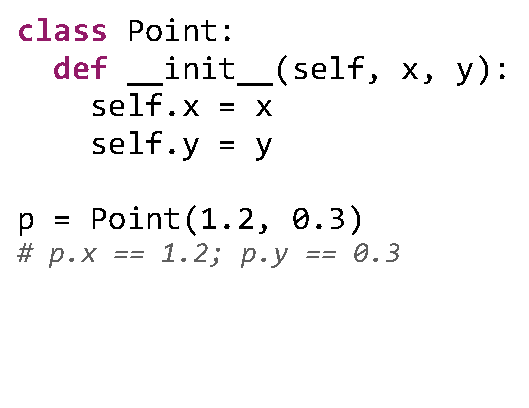
\includegraphics[scale=.7]{figures/ch5-python-class-point-code}
	\label{fig:ch5-python-class-point-code}
}
\subfigure[Generated Java class for \texttt{Point}]{
	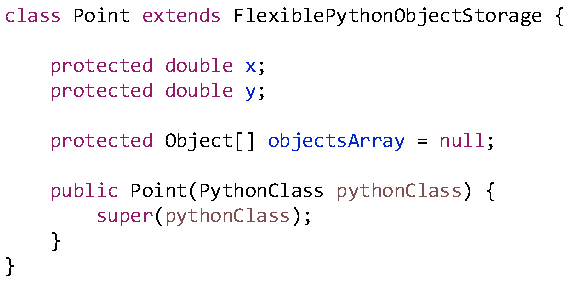
\includegraphics[scale=.95]{figures/ch5-flexible-object-storage-class-point-code}
	\label{fig:ch5-flexible-object-storage-class-point-code}
}
\caption{Flexible object storage example}
\label{fig:ch5-flexible-object-storage-example-code}
\end{figure}

In addition to the fixed object storage, ZipPy also uses a class file generation based approach to produce unique object storages for each Python class at runtime.
Figure~\ref{fig:ch5-flexible-object-storage-example-code} gives an example of the generated object storage.
As shown in Figure~\ref{fig:ch5-python-class-point-code}, the simple Python class \texttt{Point} only has two attributes, \texttt{x} and \texttt{y}.
The instantiation of \texttt{Point} shown in the Figure assigns two doubles to \texttt{x} and \texttt{y}.
Based on this type information, ZipPy generates the Java class \texttt{Point} shown in Figure~\ref{fig:ch5-flexible-object-storage-class-point-code} as the object storage for instances of the Python class.
Note that the generated Java class has two double fields to store the attributes of the Python class.
We generate the object storage class optimistically assuming that the layout of a Python \texttt{Point} object does not change in the future and the types of its attributes are also stable.
If our assumption holds, the generated Java class is the optimal object storage tailored specifically for the Python class \texttt{Point}.
In case of a layout change such as adding a new attribute or an attribute type change, the generated object storage will utilize the spill array as the fall back to accommodate new attributes.
Upon the removal of an attribute, we simply remove it from the layout table and leave the freed object storage location un-utilized.

The above mentioned object storage generation relies on layout information collected in the instantiation of the Python class.
We do not have enough information about the object layout ahead of time or before the first instantiation of the Python class at runtime.
On the other hand delaying the object storage generation results in diminishing returns, since a large number of Python objects allocated before hand cannot benefit from this optimization.
Therefore the most effective way is to generate a flexible object storage for the Python class when it first instantiated.
ZipPy uses a specialized constructor call node to perform the first instantiation of a Python class in the following steps:

\begin{enumerate}

\item Create a fixed object storage, which we refer as a bootstrapping object, to collect layout information from the constructor call.

\item Call the resolved constructor, and pass the bootstrapping object as the first argument \textsf{self}.

\item After the constructor call, generate a flexible object storage class based on the current layout of the bootstrapping object similar to the one shown in Figure~\ref{fig:ch5-flexible-object-storage-class-point-code}.

\item Create a flexible object storage using the generated storage class, and migrate the attributes from the populated bootstrapping object to the flexible object storage.

\item Rewrite the constructor call node to a version that optimizes the subsequent constructor calls by directly allocating a flexible object storage.

\item Invalidate the layout on the fixed object storage and return the instantiated flexible object storage to the caller.

\end{enumerate}

Even though we rely on a fixed object storage to bootstrap the class generation, we discard it immediately after migrating all the attributes to the flexible object storage.
Therefore, the caller of the Python constructor does not hold reference to the bootstrapping object, and it is in most cases safe to ignore it.
However, there is a special case where the bootstrapping object is accessed again.
We will discuss this issue in more detail in Section~\ref{sec:ch5-zombie-resurrection}.

Note that the bootstrapping process described above only happens once for each Python class.
After the successful generation of the flexible storage class, any subsequent attempt to instantiate the same Python class automatically picks up the updated storage class.
If the Python program does not instantiate a loaded Python class, ZipPy does not generate flexible storage class for it.

\subsection{Continuous Storage Class Generation}
\label{sec:ch5-flexible-storage-layout-evolution}

\begin{figure}
\centering
\subfigure[Extended Python class \texttt{Point}]{
	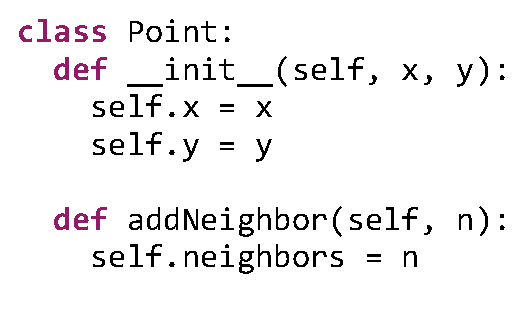
\includegraphics[scale=.7]{figures/ch5-python-class-point-with-layout-change-code}
	\label{fig:ch5-python-class-point-with-layout-changecode}
}
\subfigure[A loop that uses the \texttt{Point} class]{
	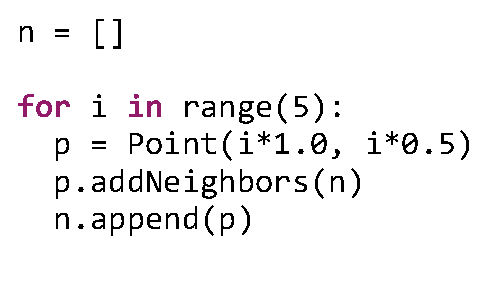
\includegraphics[scale=.7]{figures/ch5-python-class-point-used-in-loop-code}
	\label{fig:ch5-python-class-point-used-in-loop-code}
}
\caption{Python object layout change example}
\label{fig:ch5-python-object-layout-change-example-code}
\end{figure}

The above mentioned flexible object storage generation rely on a common practice among Python programmers that is do not abuse the mutability of Python objects after its instantiation.
Since it is permitted by the language, a large portion of Python programs do not strictly follow this practice.
Figure~\ref{fig:ch5-python-object-layout-change-example-code} shows an updated implementation of the Python class \texttt{Point} that changes its object layout outside the constructor.
Note that the new implementation has an additional method called \texttt{addNeighbors}.
The method inserts a new attribute to the instances of \texttt{Point}.
A hypothetical loop shown in Figure~\ref{fig:ch5-python-class-point-used-in-loop-code} calls the \texttt{addNeighbors} method in the loop body, and causes a layout change after the instantiation of the class \texttt{Point}.
The behavior of the program shown in the Figure does not follow the suggested coding practice, however, it is in fact commonplace among Python programs.

Although flexible object storage is capable of handling layout changes like the one shown in Figure~\ref{fig:ch5-python-object-layout-change-example-code}, it does so by spilling the new attribute to the spill array.
A few number of layout changes occurred after the instantiation is enough to cripple the performance advantage of using such a flexible object storage.
To address this issue we extended flexible object storage generation in ZipPy to support continuous generation of storage classes.
Every newly generated storage class adopts the layout changes happened so far.
So if the layout changes converge to a stable point, ZipPy allocates all subsequently instantiated Python objects using the optimal flexible object storage.

\begin{figure}
\centering
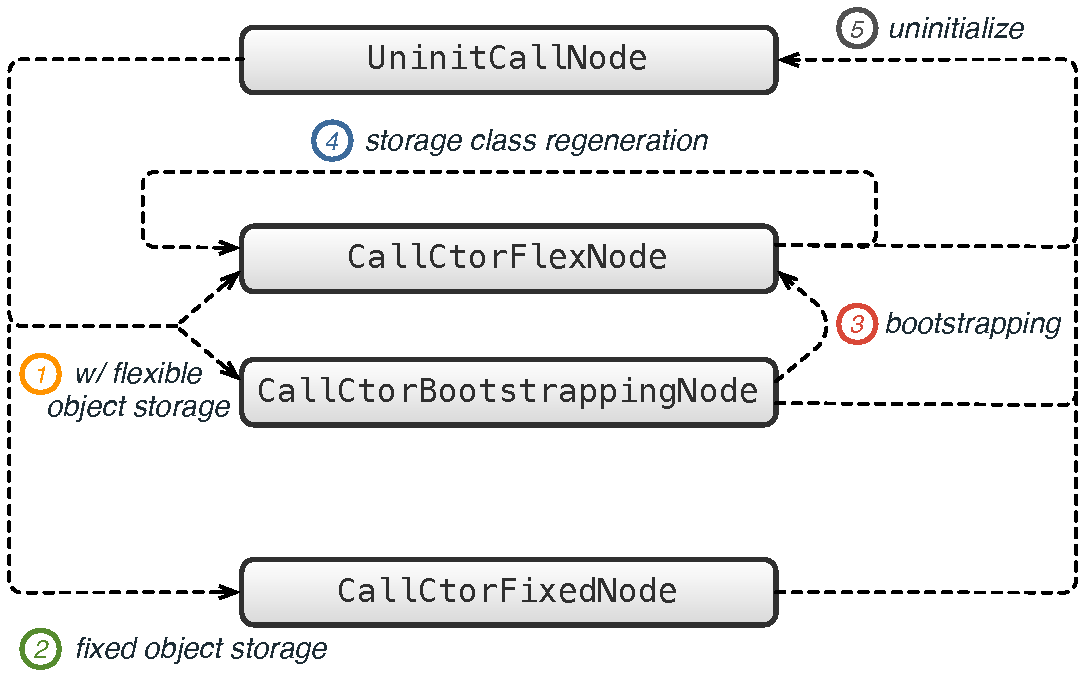
\includegraphics[scale=.65]{figures/ch5-constructor-call-site-transformation}
\caption{Constructor call site transformation}
\label{fig:ch5-constructor-call-site-transformation}
\end{figure}

ZipPy supports continuous storage class generation by applying a series of node transformations on a constructor call site.
We implement a number of call node versions specifically for constructor calls or constructor call nodes.
Each version handles the allocation of the new Python object in a different way.
Figure~\ref{fig:ch5-constructor-call-site-transformation} shows the various call constructor nodes in ZipPy.
The descriptions of each node is as follows:

\begin{itemize}

\item \texttt{UninitCallNode}: Uninitialized call node representing an un-executed call site.

\item \texttt{CallCtorFlexNode}: Specialized constructor call node that allocates Python object instances using a flexible object storage.

\item \texttt{CallCtorBootstrappingNode}: Specialized constructor call node that bootstraps the initial flexible storage class generation.

\item \texttt{CallCtorFixedNode}: Specialized constructor call node that allocates Python object instances using a fixed object storage.

\end{itemize}

Figure~\ref{fig:ch5-constructor-call-site-transformation} also illustrates the transformations between different call constructor nodes that enables continuous storage class generation.
The descriptions of the transformation rules are as follows:

\begin{enumerate}

\item With flexible object storage enabled, upon the first execution of a constructor call site, ZipPy rewrites the uninitialized call node to a constructor call node that allocates flexible object storages.
If this call is the first instantiation of the target Python class, we rewrite the call node to a \texttt{CallCtorBootstrappingNode}.
Otherwise, if the target Python class has an existing flexible storage class, we rewrite the call node to a \texttt{CallCtorFlexNode}.

\item With flexible object storage disabled, the initialization of a constructor call site rewrites the call node simply to a \texttt{CallCtorFixedNode}.

\item After the first instantiation of a Python class, the \texttt{CallCtorBootstrappingNode} generates the first flexible storage class and rewrites itself to a \texttt{CallCtorFlexNode}.

\item When a \texttt{CallCtorFlexNode} detects a layout change, it generates an updated Java storage class for the target Python class, and allocates a Python object using the updated storage class.
It also rewrites itself to a new \texttt{CallCtorFlexNode} optimizing for the allocation of the updated storage class.

\item If the callee of the constructor call changes, all specialized call node transforms back to the uninitialized call node.

\end{enumerate}

Each Python class keeps track of its own Java storage classes used to instantiate the Python class.
It marks the most recently generated storage class as its current storage class.
Each \texttt{CallCtorFlexNode} caches the current storage class and the Java method handle~\cite{jdk8} of its constructor.
When allocating an object storage, the \texttt{CallCtorFlexNode} calls the Java constructor of the storage class by using the cached method handle.
A Python object layout change signals its Python class to mark the current storage class as ``old''.
The following instantiation of the Python class triggers an storage class generation, and replaces the ``old'' current storage class with the ``new'' one.
Subsequent instantiations of the Python class automatically pick up the update, and make sure to allocate Python object instances using the current storage class.

\subsection{A Generalization to the Object Model}

\begin{figure}
\centering
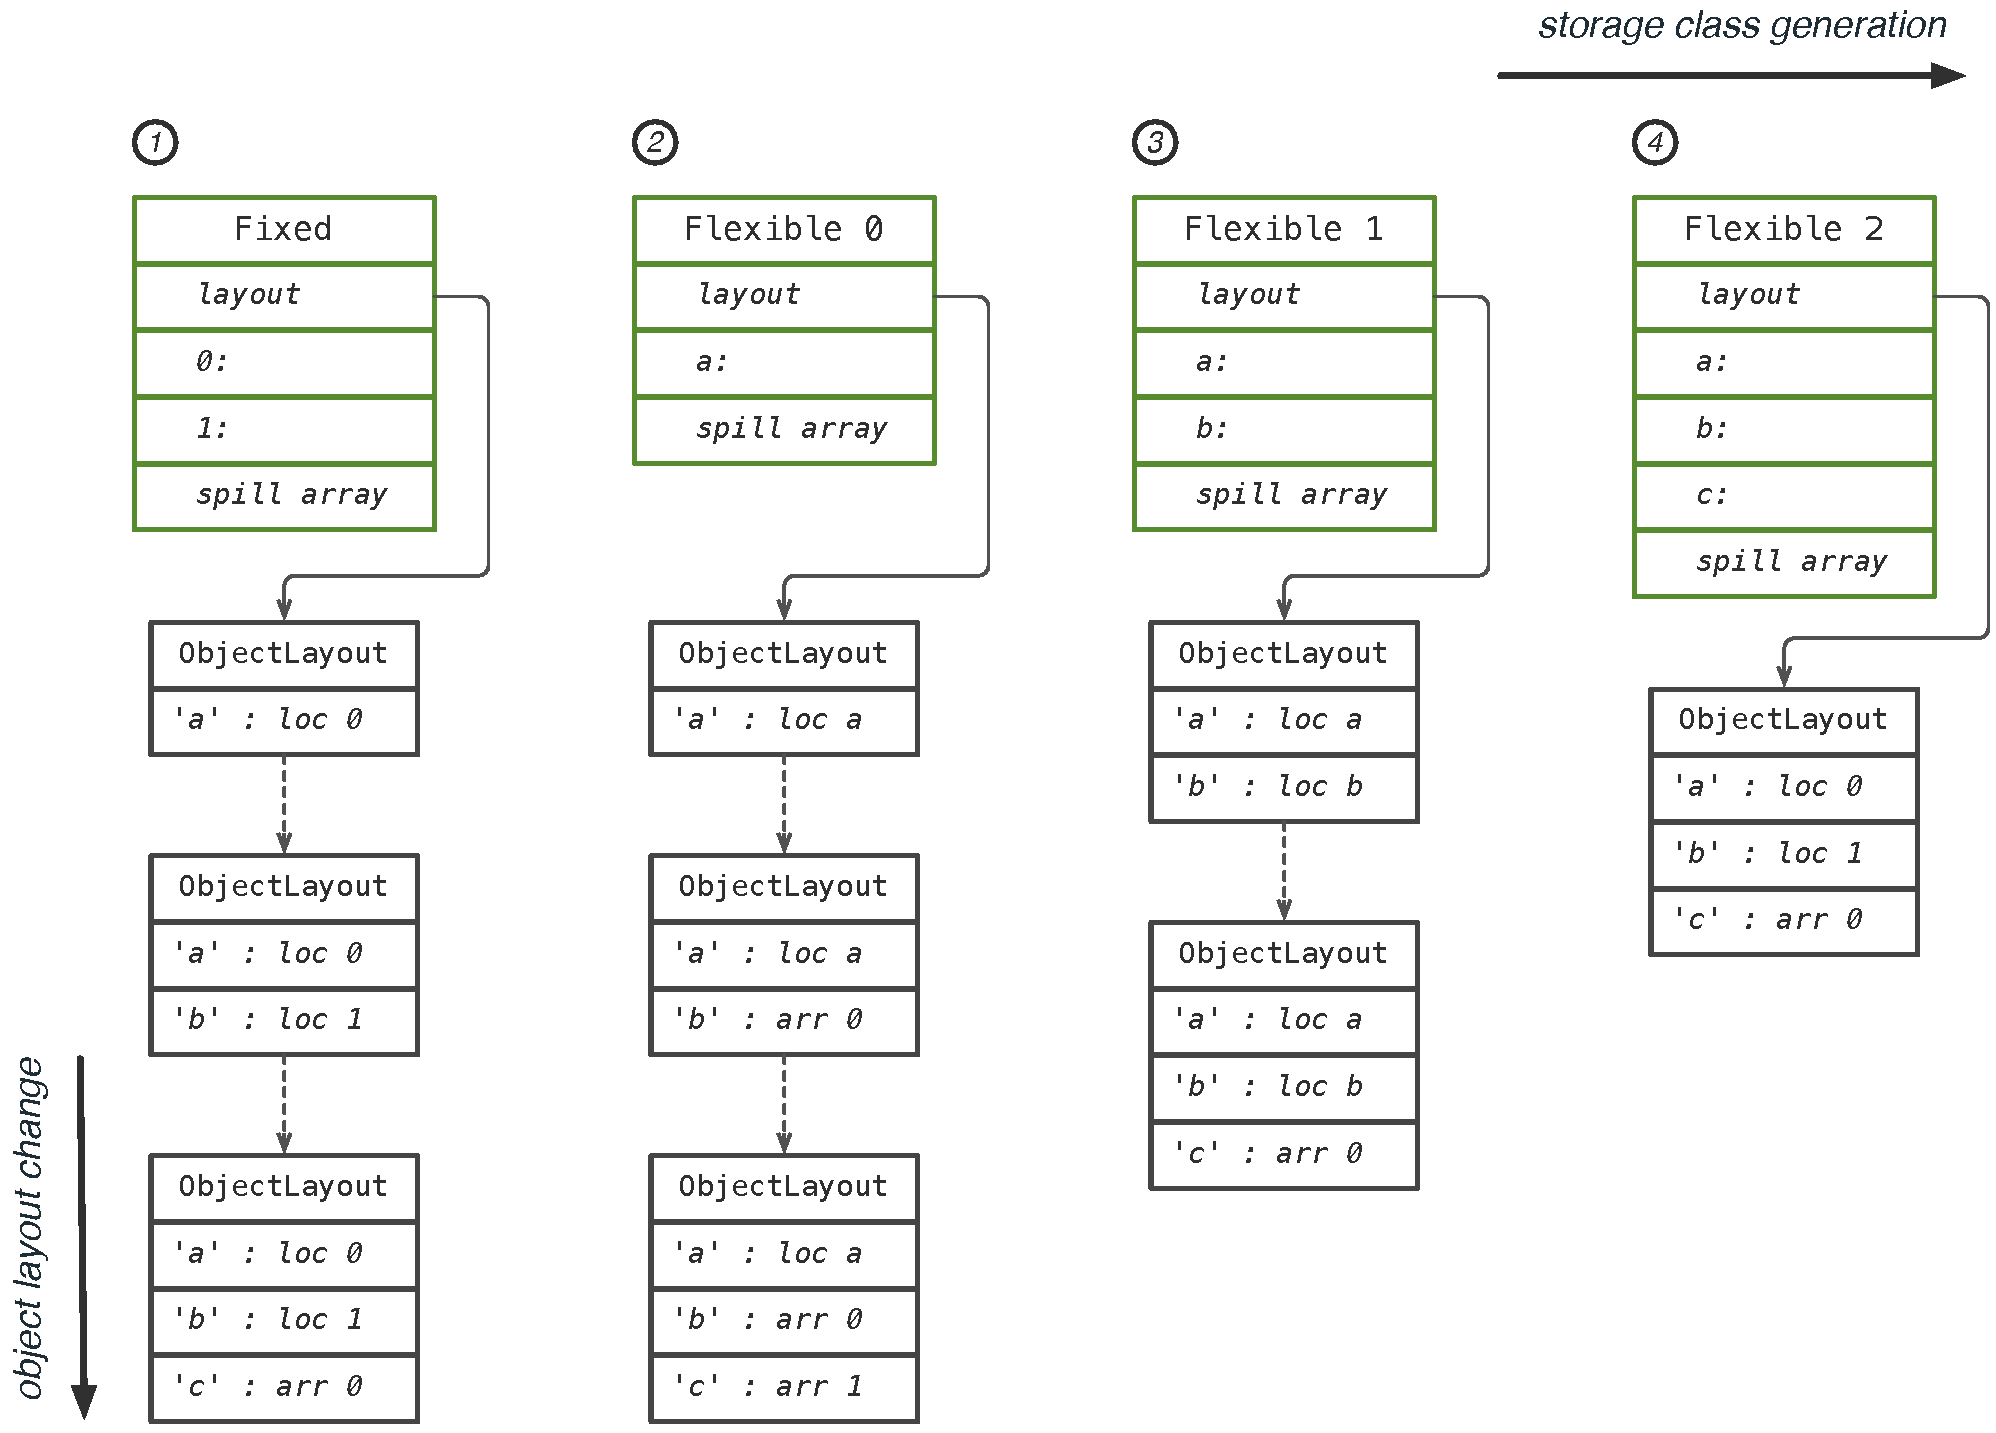
\includegraphics[scale=.49]{figures/ch5-object-storage-class-generation-and-object-layout-change}
\caption{Continuous storage class generations and object layout changes of an example Python class}
\label{fig:ch5-object-storage-class-generation-and-object-layout-change}
\end{figure}

Continuous storage class generation generalizes the existing object model of ZipPy to enable the use of multiple storage classes for a single Python class.
Figure~\ref{fig:ch5-object-storage-class-generation-and-object-layout-change} illustrates the transitions of storage classes and object layouts of an example Python class during the life time of the class.
In the object model described previously where we only use fixed storage classes to model Python objects, an object layout change at runtime triggers a transition vertically in the Figure.
Whereas with continuous storage class generation an object layout change also triggers a storage class regeneration along the horizontal direction in the Figure.
The transitions of the storage classes are orthogonal to that of the object layouts.
Each storage class follows its own object layout transitions.

Every Python object has its own life time.
The life time starts from the instantiation of the object, and ends at the point that it is not referenced by the program and ready to be garbage collected.
In the middle of its life time, a Python object allocated using on storage class in general cannot migrate its attributes to use another storage class.
Since there could be existing pointers that reference the current object storage of the Python object, a storage class migration will turn those existing pointers into dangling pointers.
Therefore, a Python object needs to reside in a single object storage throughout its life time.

A storage class generation caused by an object layout change only benefits Python objects instantiated after the layout change.
The living or existing objects of the same Python class handle layout changes lazily by spilling the new attribute to the spill array and updating its own layout table.
Note that similar to the fixed object layout approach, we synchronize object layout changes across all the Python objects allocated using the same storage class.
We will use a program execution example to further explain the object layout synchronizations.
For instance, along the execution of a hypothetical Python program, the program at one point allocates two Python object \textsf{A} and \textsf{B} both using the storage class \texttt{Flexible 0} shown in Figure~\ref{fig:ch5-object-storage-class-generation-and-object-layout-change}.
Since Python object instantiation always picks up the latest storage class, \texttt{Flexible 0} is the most current storage class at this point.
Both \textsf{A} and \textsf{B} only have a single attribute \texttt{a}.
At a later point, an object layout takes place by adding an attribute \texttt{b} to the object \textsf{A}.
Object \textsf{A} updates its own layout table, invalidates the previous object layout, and sets the new object layout as the valid layout of \texttt{Flexible 0}.
Since we invalidated the previous object layout, any object that still uses the old layout needs to \emph{synchronize} to the updated layout.
The following access to object \textsf{B} will cause an slow path execution that synchronizes its object layout with \texttt{Flexible 0}.
After the layout synchronization, even though object \textsf{B} does not actually contain the attribute \texttt{b}, its layout table includes an entry for \texttt{b}.
Note that the above mentioned layout change also signals the Python class to generate storage class \texttt{Flexible 1}.
However, object \textsf{A} and \textsf{B} will not migrate to another storage class and always synchronize its with \texttt{Flexible 0} to share the same object layout.

Object layout synchronization simplifies the attribute access dispatch we explained in Section~\ref{sec:ch5-attribute-access-dispatch-chain}.
It ensures that we only need to maintain a single valid cache entry to access Python objects allocated using the same storage class.
However, in its life time, a Python class could generate multiple storage classes.
It is inevitable that at the same program location we need to built multiple cache entries, one for each storage class, to optimize accesses to Python objects of the same class.

\subsection{Zombie Resurrection}
\label{sec:ch5-zombie-resurrection}

\begin{figure}
\centering
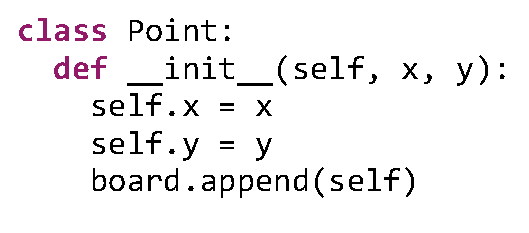
\includegraphics[scale=.7]{figures/ch5-python-class-point-with-zombie-store-code}
\caption{A Python constructor that exposes a reference to \texttt{self}}
\label{fig:ch5-python-class-point-with-zombie-store-code}
\end{figure}

We uses a fixed object storage to bootstrap the initial storage class generation.
But we only return the instantiated Python object to the caller of the constructor after migrating to a flexible object storage and discarding the initial fixed one.
This approach ensures that the consumer of the constructor call only references the flexible object storage.
However, there are cases where the constructor itself could expose the reference to the fixed object storage making it accessible outside the constructor.
Figure~\ref{fig:ch5-python-class-point-with-zombie-store-code} shows a modified definition of the Python class \texttt{Point}.
The constructor of \texttt{Point} stores a reference to \texttt{self} to the Python list \texttt{board}.
The reference store makes potential accesses to \texttt{self} possible outside the constructor.
So during the storage class bootstrapping of \texttt{Point}, the shown reference store of \texttt{self} will make the bootstrapping object modeled using the fixed object storage accessible at a later point.
We refer this scenario as zombie resurrection.
Since the bootstrapping object, in most case a \emph{dead} object, comes to live again in this particular situation.

We address this issue by turning the zombie object storage into a proxy to the flexible storage object it migrates to.
To be more specific, in the last step of bootstrapping a storage class generation, after migrating to the flexible object storage, we pass a reference to the flexible object storage the zombie object storage, and flag it as a proxy.
As a proxy, the zombie redirects all attribute accesses to the flexible object storage.
This approach ensures that all references to the first instance of a Python class eventually access the same flexible object storage, hence, preserves the correct semantics.

\subsection{Discussion}

ZipPy execute Python programs first in the interpreter mode, and compiles the program when it becomes hot.
The warming up phase of the guest program executes in interpreter mode.
ZipPy compiles the Python program only after it has been executed for a few iterations when the specializations of the program become stable.
The same type locality principle applies to Python object layouts as well.
That is the layouts of Python objects of the same class tend to converge and stabilize after the initial warm up phase.
Therefore, ZipPy in most cases compiles Python programs only after their object layout evolution has stabilized.
The underlying Java JIT compiler treats Python objects as regular Java objects, since we model them using ordinary Java objects.
The compiler is able to apply aggressive optimizations such as escape analysis to Python objects as well.
When combined with flexible storage class generation, our object model design offers both performance and space efficiency that closes the gap between the guest language and the host language.
